% Copyright (c) 2014,2016,2018 Casper Ti. Vector
% Public domain.

\chapter{晶胞中原子重叠的实时检测和排除}\label{chap:cryst-cd}
\section{晶体学粗碰撞检测}

对物体重叠的检测属于计算几何中的\myterm{碰撞检测}(collision detection)问题%
\parencite{ericson2005},所以为了在全局最优化中高效地实时检测和排除存在原子重叠
的晶体模型,首先需要的就是一种实时的晶体学碰撞检测算法。对于含 $n$ 个原子的晶
胞,如果通过直接逐对计算原子间距来检测重叠,那么就须要计算所有 $n (n - 1) / 2$
个原子对的间距,因此算法的时间复杂度为 $O(n^2)$ 量级;由此可见 $n$ 较大时逐对
算法在性能上是不利的,而这一问题也是实现实时碰撞检测的主要障碍之一。为了解决
这一问题,实际的碰撞检测通常被分为\myterm{粗碰撞检测}(broad phase)和%
\myterm{细碰撞检测}(narrow phase)两个步骤\parencite[329]{ericson2005}:
前者排除那些明显不会发生碰撞的物体对,而后者对剩下的物体对进行精确的测试
以判断其是否发生碰撞。本节主要就粗检测展开讨论。

\subsection{晶胞的几何构造}\label{ssec:cryst-geom}

对于直角坐标系下的低维 Euclid 空间,碰撞检测是较为成熟的研究领域;然而晶胞有其
独特的几何构造,这使我们难以在晶胞中原封不动地应用现有的碰撞检测算法。首先的
问题是晶胞的 $a$、$b$、$c$ 轴在很多情况下并不互相正交,因此在晶胞中常常不便使用
直角坐标系;针对这一问题,晶体学家的惯用对策是使用分数坐标。假设晶胞中某位移向量
$\vec{x}$ 的分数坐标为 $\mat{x} = (x, y, z)^\tee$,则其 Cartesian 坐标为
\begin{equation}
	\mat{r} = x\mat{a} + y\mat{b} + z\mat{c}
	= \big(\mat{a}\ \mat{b}\ \mat{c}\big) {
		\renewcommand*{\arraystretch}{0.66}
		\begin{pmatrix} x \\ y \\ z\\\end{pmatrix}
	} = \mat{A}\mat{x}\mccomma
\end{equation}
其中 $\mat{a}$、$\mat{b}$、$\mat{c}$ 为正空间各基向量的 Cartesian 坐标。
可见坐标变换矩阵 $\mat{A}$ 正是基向量组矩阵,且进一步可知 $\vec{x}$ 的长度为
\begin{equation}
	\mat{r}^\tee\mat{r} = \mat{x}^\tee\mat{A}^\tee\mat{A}\mat{x}
	= \mat{x}^\tee\mat{G}\mat{x}\mccomma
\end{equation}
其中二次型 $\mat{G} = \mat{A}^\tee\mat{A}$ 正是分数坐标下以矩阵形式表示的
晶胞度规张量\parencite[66]{dodson1991},而后者决定了晶胞中的距离构造。
在分数坐标下,晶胞中的原子位置可以用 3 个互相独立的坐标 $x$、$y$、$z$ 表示;
又因为每个坐标分别满足周期边界条件,即它们各是一个一维圆环 $S^1$ 上的坐标,
所以分数坐标下的晶胞事实上是被建模为 3 个一维圆环的 Cartesian 积(类似于图
\ref{fig:torus-period} 中的情形),即一个三维环面 $T^3$%
\parencite{choquet2009},而这个三维环面具有上述的特殊距离构造。

\begin{figure}[htbp!]\bfcmd
\ffigbox{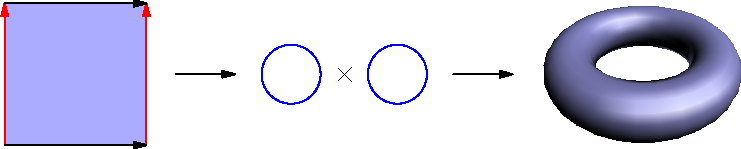
\includegraphics[width = 0.7\textwidth]{img/torus-period}}{\caption{%
	二维晶胞建模为二维环面:$S^1 \times S^1 = T^2$%
}\label{fig:torus-period}}
\end{figure}

粗碰撞检测中一种很普遍的做法是围绕每个被检测的物体构造一个包围体%
\parencite[75-123]{ericson2005},然后利用包围体的特定几何属性来进行优于
$O(n^2)$ 的粗检测;一种常用的包围体是\myterm{轴对齐包围盒}(axis-aligned
bounding box,简称 AABB),即以物体在各坐标轴上的投影区间为边界的盒子(图
\ref{fig:aabb-frac})。两个 AABB 间发生碰撞当且仅当其在 3 个坐标轴上的投影区间
均发生碰撞,因此使用 AABB 在很多时候可以将三维问题化为 3 个一维问题;注意到这里
应用的是变量分离的数学思想,而在晶胞内用分数坐标正好可以实现 3 个坐标的分离,
在使用 AABB 对晶胞内原子进行粗检测时使用分数坐标显然是最合适的选择\footnote{%
	此外,因为上述的 AABB 碰撞判据只涉及对投影区间上下界的比较而不涉及距离,
	所以分数坐标下晶胞的特殊距离构造并不影响 AABB 的使用。%
}。最后,为了能使用 AABB 进行粗检测,还须要解决计算 AABB 的问题:具体而言,
给定原子的分数坐标和 Cartesian 半径 $r$,如何计算其在分数坐标下的 AABB?

\begin{figure}[htbp!]\bfcmd
\ffigbox%
	{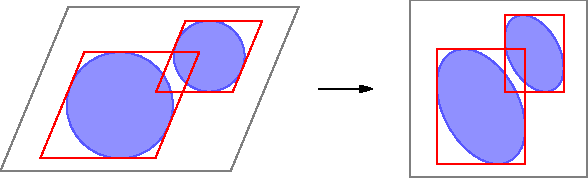
\includegraphics[width = 0.6\textwidth]{img/aabb-frac}}%
	{\caption{轴对齐投影和分数坐标下 AABB 的等价性}\label{fig:aabb-frac}}
\end{figure}

考虑到分数坐标下使用 AABB 正好等价于在以 $a$、$b$、$c$ 轴为坐标轴的仿射坐标下
使用和坐标轴对齐的斜投影(图 \ref{fig:aabb-frac}),不妨从一个和 $a$ 轴及 $a^*$
轴均正交(因此也和 $bOc$ 平面平行)的方向考察上述原子在 $a$ 轴上的轴对齐投影
(图 \ref{fig:aabb-width-1}),此时只须计算投影区间的半宽 $R$ 即可。
根据相似三角形的性质可知
\begin{equation}
	\frac{R}{a} = \frac{r}{d} \Rightarrow
	\frac{R}{ar} = \frac{1}{d} = a^* = \frac{\sin\alpha}{av}\mccomma
\end{equation}
其中 $d$ 为相邻两 $bOc$ 晶面的间距,而
\begin{equation}
	v = V / abc = \sqrt{
		1 - \cos^2 \alpha - \cos^2 \beta - \cos^2 \gamma
		+ 2 \cos\alpha \cos\beta \cos\gamma
	}
\end{equation}
为晶胞的无量纲化体积;$a^*$ 和 $V$ 的计算公式引自文献%
\parencite[1-4]{prince2004}。在实际的粗检测中使用的是分数坐标,
因此最终用到的半宽应为
\begin{equation}
	\frac{R}{a} = \frac{r}{d} = \frac{r\sin\alpha}{av}\mcscolon
\end{equation}
同理可对 $b$、$c$ 轴得到类似的结论。

\begin{figure}[htbp!]\bfcmd
\setlength{\columnsep}{2.5em}
\begin{floatrow}
	\ffigbox[0.4\textwidth]%
		{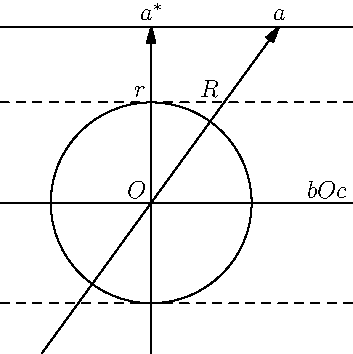
\includegraphics[width = 0.32\textwidth]{img/aabb-width-1}}%
		{\caption{原子在 $a$ 轴上的轴对齐投影}\label{fig:aabb-width-1}}
	\ffigbox[0.4\textwidth]%
		{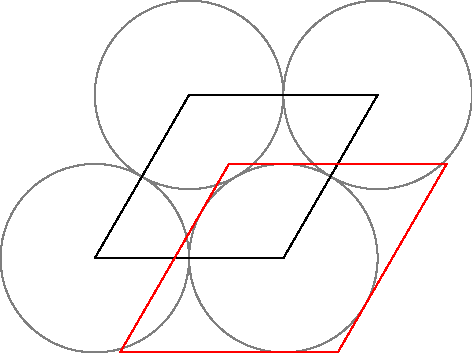
\includegraphics[width = 0.28\textwidth]{img/aabb-width-2}}%
		{\caption{一种 AABB 比晶胞大的情形}\label{fig:aabb-width-2}}
\end{floatrow}
\end{figure}

晶胞的周期边界也会影响碰撞检测,但考虑到 $T^3$ 是三维流形,流形的概念%
\parencite[161]{dodson1991}可以给我们一定的启发:可以把看成盒子的晶胞
强行分为“边界”和“内部”两部分,其内部完全类似于具有非平凡 Euclid 度规张量的
普通空间。因此,对于完全包含于晶胞内部的 AABB,可以按常规流程进行粗碰撞检测,
不用担心受周期边界的影响;而对于跨边界的 AABB,我们须要进行专门的额外检测。

\subsection{晶胞中的 sweep and prune}\label{ssec:cryst-sap}

在使用轴对齐包围盒(AABB)的碰撞检测算法中,利用树状数据结构的算法,如
\textcite{grudinin2010}的算法可以考虑已有的成键信息,因此特别适合处理成键关系
大部分已知的结构;对于成键关系总体未知的结构,我们需要的是能从头检测碰撞的算法,
而这类算法中一种最简单的是 \myterm{sweep and prune}(简称 SAP,也称为 sort and
sweep;参考 \cite[329-338]{ericson2005})。假设我们希望在非周期边界的前提下检测
$n$ 个物体(例如图 \ref{fig:sap-sweep-1} 中的那些)之间的碰撞;在 SAP 算法中,
我们会首先将物体投影到某个方便使用的坐标轴上,然后对投影区间进行碰撞检测:

\begin{figure}[htbp!]
\ffigbox%
	{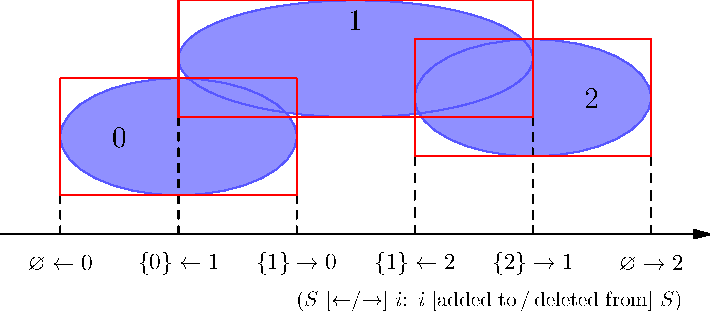
\includegraphics[width = 0.7\textwidth]{img/sap-sweep-1}}%
	{\caption{非周期边界 SAP 算法示例}\label{fig:sap-sweep-1}}
\end{figure}

\begin{itemize}
\item 将各投影区间的上下界在排序后存入一个列表 $l$(sort 步骤),
	然后建立一个空集 $S$,并通过从小到大扫描 $l$ 中的各个上下界来
	跟踪各上下界处投影区间之间的碰撞(sweep 步骤)。
\item 当扫描到一个下界时,报告相应投影区间和 $S$ 中每个区间的碰撞,
	然后将该区间插入 $S$ 中:例如在图 \ref{fig:sap-sweep-1} 中,
	当扫描到区间 \#1 的下界时,算法会先报告区间 \#0 和 \#1 之间的碰撞,
	然后将区间 \#1 插入 $S$ 中。
\item 当扫描到一个上界时,从 $S$ 中删除相应的投影区间:例如在图
	\ref{fig:sap-sweep-1} 中,当扫描到区间 \#1 的下界时,
	该区间会被从 $S$ 中删除。
\end{itemize}

在 SAP 中,$S$ 上的插入和删除操作常常并入和 SAP 的输出(报告)代码,
因此习惯上并不在粗检测的复杂度分析中考虑\parencite[333]{ericson2005}。
虽然如此,不难注意到这些操作的总复杂度取决于实际发生碰撞的物体对数:
如果每个物体都和其它所有物体发生碰撞,那么 $S$ 上的插入和删除操作无论如何
都将至少花费 $O(n^2)$ 时间。如果 sort 步骤中使用的是合适的排序算法,
例如归并排序\parencite[158-168]{knuth1998},则该步骤花费的时间在最坏的
情形下也是 $O(n\log n)$ 量级;而 sweep 步骤花费的时间显然是 $O(n)$ 量级,
所以 SAP 的总时间复杂度可以为 $O(n\log n)$ 量级。

如第 \ref{ssec:cryst-geom} 小节所述,晶胞中周期边界对粗碰撞检测算法的影响
往往可以通过对跨边界的 AABB 进行专门的额外检测来解决。就 SAP 而言,因为其
正确性依赖于每个投影区间的下界在上界之前被扫描到,周期边界所带来的问题
在于跨边界区间的上半部分在 sweep 步骤中会被算法错误地忽略:例如在图
\ref{fig:sap-sweep-2} 中,区间 \#0 的上半部分和区间 \#1 之间的碰撞就被
忽略了。然而考虑到在 sweep 步骤的末尾,集合 $S$ 中会包含所有的跨边界区间,
我们可以对常规的 SAP 算法进行如下的修改:

\begin{figure}[htbp!]
\ffigbox%
	{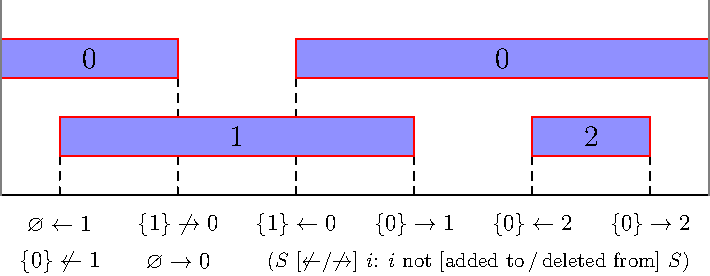
\includegraphics[width = 0.7\textwidth]{img/sap-sweep-2}}%
	{\caption{周期边界下 SAP 算法示例}\label{fig:sap-sweep-2}}
\end{figure}

\begin{itemize}
\item 执行原 SAP 算法的步骤,但当扫描到上界时须要注意,如果相应的下界尚未遇到,
	那么它们所对应的投影区间将不在集合 $S$ 中,因此试图从 $S$ 中删除相应区间
	将是无意义的。例如在图 \ref{fig:sap-sweep-2} 中,当扫描到区间 \#0 的上界时,
	我们不能从 $S$ 中删除该区间。
\item 原步骤执行完之后,再次从小到大扫描列表 $l$,但不在 $S$ 中插入区间:
	跨边界区间互相之间的碰撞在原 sweep 步骤的末尾已被处理,所以我们只关心
	不跨边界的区间和跨边界区间之间的碰撞。例如在图 \ref{fig:sap-sweep-2}
	中,再次扫描到区间 \#1 的下界时,该区间不会被插入 $S$ 中。
\item 当 $S$ 成为空集时,算法终止。例如在图 \ref{fig:sap-sweep-2} 中,
	再次扫描到区间 \#0 的上界时,算法终止。
\end{itemize}

上述改动中额外加入的新 sweep 步骤在在最坏的情形下将花费 $O(n)$ 量级的时间,
因此修改后 SAP 算法的时间复杂度仍可以为 $O(n\log n)$。在此基础之上有必要指出,
为了正确、高效地实现 SAP,一些技术细节须要特别注意:

\begin{itemize}
\item 在上述新加的 sweep 步骤中,部分碰撞对有可能会被重复报告,例如图
	\ref{fig:sap-sweep-2} 中区间 \#0 和 \#1 之间的碰撞会被报告两次,
	而这些重复的报告应该在实现时加以正确处理。
\item 上述改动通过判断投影区间的下界是否小于上界来检测跨边界区间,但这样的做法
	在区间长度不小于坐标轴的长度时(例如图 \ref{fig:aabb-width-2} 中的情形)
	会出错。为了处理这种情形,可以强行限制区间在分数坐标下的半宽最多为
	$0.5 - \varepsilon$,其中 $\varepsilon > 0$ 为一很小的常数。
\item 在 $n$ 很大的情形下,如果只在一个坐标轴上使用 SAP,碰撞对可能不会被有效
	筛除:例如在图 \ref{fig:mult-axes}(a) 中,只在 $x$ 或 $y$ 轴上使用 SAP
	都不能有效筛除碰撞对;此时在多个坐标轴上使用 SAP\footnote{%
		顺便指出,在使用多坐标轴 SAP 时正相当于构造了以物体在各坐标轴上的投影
		区间为边界的盒子,即物体的 AABB,因此 SAP 被分类为使用 AABB 的算法。%
	} 有可能会实现更高的总体性能(但也未必,参考第 \ref{ssec:cd-eval} 小节)。
\item 被检测物体在特定坐标轴上的投影区间可能特别拥挤,例如图
	\ref{fig:mult-axes}(b) 中的 $x$ 轴;此时在这些轴上使用 SAP 效果将很差,
	因此在 SAP 中可以跳过这些轴。由第 \ref{ssec:cryst-geom} 小节可知,
	在 $R/ar$ 值特别大的坐标轴上容易出现拥挤问题,
	因此在晶胞中使用 SAP 时建议不用这些轴。
\item 在物理建模中,往往可以认为一对只在彼此边界上发生碰撞的物体(例如一对
	相切的球)并不真正发生相互作用;因此如果一些上下界在 $l$ 中排名相同时,
	可以先处理上界,然后处理下界。
\item 快速排序算法\parencite[113-122]{knuth1998}在最坏情形下具有 $O(n^2)$
	的复杂度,但其平均复杂度仍为 $O(n\log n)$,且常数因子更小(参考第
	\ref{ssec:incr-intro} 小节),因此其比归并排序更适用于 SAP 中的 sort 步骤。
\end{itemize}

\begin{figure}[htbp!]\bfcmd
\ffigbox{\begin{subfloatrow}
	\setlength{\columnsep}{2em}
	\ffigbox[\FBwidth]%
		{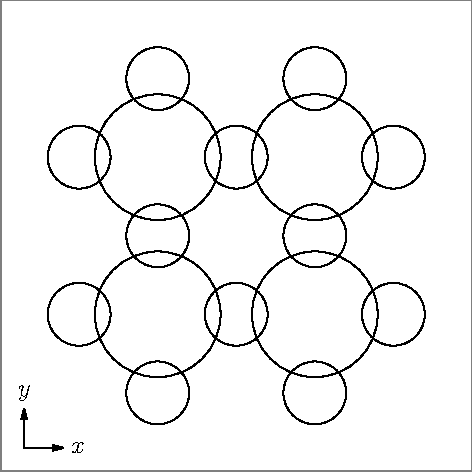
\includegraphics[height = 0.3\textwidth]{img/mult-axes-1}}%
		{\caption{一种单坐标轴 SAP 效果较差的情形}}
	\ffigbox[0.2\textwidth]%
		{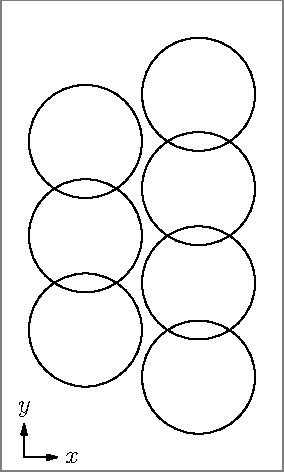
\includegraphics[height = 0.3\textwidth]{img/mult-axes-2}}%
		{\caption{一种应跳过 $x$ 轴上 SAP 的情形}}
\end{subfloatrow}}{\caption{SAP 实现中一些技术细节的示例}\label{fig:mult-axes}}
\vspace{\slop{-0.5em}}
\end{figure}

最后,考虑到因为 Coulomb 相互作用,两个原子间的正常键长可能不同于其半径之和,
我们引入\myterm{对缩放因子}(pairwise zoom factor)$p$ 的概念,其定义为
上述正常键长和半径之和的比。此外我们定义原子的\myterm{碰撞检测半径}%
(collision-detection radius)为用来计算其投影区间的半径,其等于原子的
正常半径 $r_0$ 乘以其\myterm{原子缩放因子}(atomic zoom factor)$q$。
显然,为了保证粗检测的正确性,对任意的原子对 $\{k_0, k_1\}$ 应有
\begin{equation}
	p(k_0, k_1) (r_0(k_0) + r_0(k_1)) \leq
	q(k_0) r_0(k_0) + q(k_1) r_0(k_1)\mcstop
\end{equation}

\subsection{利用等效点系对称性简化粗碰撞检测}\label{ssec:ep-sym}

因为等效点系组合法(参考第 \ref{sec:dspace-epc} 节)的使用,我们可以利用
等效点系对称性来降低晶胞粗碰撞检测的复杂度,而本节将就此进行讨论。
为了方便推导,首先约定用下标 $i$ 标记晶胞中的独立原子,其中 $i = 0, 1,
\cdots, m - 1$;用下标 $ij$ 标记独立原子 $i$ 的等效原子,其中 $j = 0, 1,
\cdots, n_i - 1$:例如在图 \ref{fig:eq-eval-1} 中,第 1 个独立原子的
第 2 个等效原子被标记为 $01$($i = 0$,$j = 1$)。考虑一个两体函数
\begin{equation}
	c(i_0j_0, i_1j_1) = c(i_1j_1, i_0j_0)\quad(i_0j_0 \neq i_1j_1)\mccomma
\end{equation}
该函数满足\myterm{等效点系对称性}:对于任何兼容于上述晶胞的对称操作 $T$,有
\begin{equation}
	c(i_0j_0, i_1j_1) = c(T(i_0j_0), T(i_1j_1))\mcscolon
\end{equation}
例如 Euclid 距离函数和第 \ref{ssec:eval-func}
小节中的对势函数(图 \ref{fig:eq-eval-2})都满足这一条件。

\begin{figure}[htbp!]\bfcmd
\setlength{\columnsep}{3em}
\begin{floatrow}
	\ffigbox[\FBwidth]%
		{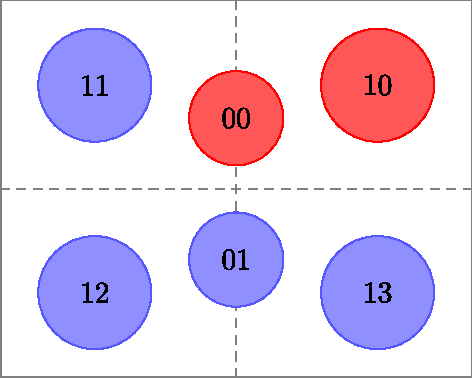
\includegraphics[width = 0.32\textwidth]{img/eq-eval-1}}%
		{\caption{等效点系对称性示例}\label{fig:eq-eval-1}}
	\ffigbox[\FBwidth]{%
		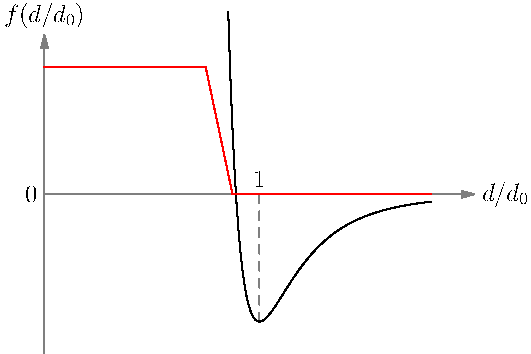
\includegraphics[width = 0.45\textwidth]{img/eq-eval-2}%
	}{%
		\captionsetup{width = 0.4\textwidth}%
		\caption[实际使用的对势和 Lennard-Jones 势的对比]%
			{实际使用的对势(浅色)和 Lennard-Jones 势(深色)的对比}%
		\label{fig:eq-eval-2}%
	}
\end{floatrow}
\end{figure}

对于任意原子 $i_0j_0$,由等效原子的定义可知必然存在一对称操作
$T_{i_0j_0}$ 将其变换为原子 $i_00$,于是有
\begin{equation}
	\sum_{i_1j_1 \neq i_0j_0}\hspace*{-1.5ex} c(i_0j_0, i_1j_1)
	= \hspace*{-1.5ex}\sum_{i_1j_1 \neq i_0j_0}\hspace*{-1.5ex}
		c(i_00, T_{i_0j_0}(i_1j_1))
	= \hspace*{-1.1ex}\sum_{i_1j_1 \neq i_00}\hspace*{-1.1ex} c(i_00, i_1j_1)
	\mccomma
\end{equation}
因此进一步有
\begin{equation}
	\sum_{\{i_0j_0, i_1j_1\}}\hspace*{-1.9ex} c(i_0j_0, i_1j_1)
	= \frac12\sum_{i_0} n_{i_0}
		\hspace*{-1.1ex}\sum_{i_1j_1 \neq i_00}\hspace*{-1.1ex} c(i_00, i_1j_1)
	= \hspace*{-1.9ex}\sum_{\{i_0j_0, i_1j_1\}}\hspace*{-1.9ex}
		\delta_{j_0} n_{i_0} c(i_0j_0, i_1j_1)\mccomma
\end{equation}
其中
\begin{equation}
	\delta_j = \left\{\,{
		\renewcommand*{\arraystretch}{0.75}
		\begin{matrix}
			1 &	(j = 0) \\
			0 &	(j \neq 0) \\
		\end{matrix}
	}\right.
\end{equation}
为 Kronecker 记号。

由此又有
\begin{equation}
	\sum_{\{i_0j_0, i_1j_1\}}\hspace*{-1.9ex} c(i_0j_0, i_1j_1)
	= \hspace*{-1.9ex}\sum_{\{i_0j_0, i_1j_1\}}\hspace*{-1.9ex} c(i_1j_1, i_0j_0)
	= \hspace*{-1.9ex}\sum_{\{i_0j_0, i_1j_1\}}\hspace*{-1.9ex}
		\delta_{j_1} n_{i_1} c(i_0j_0, i_1j_1)\mcscolon
\end{equation}
两式平均即得最终用到的关系
\begin{equation}
	C = \hspace*{-1.9ex}\sum_{\{i_0j_0, i_1j_1\}}\hspace*{-1.9ex} c(i_0j_0, i_1j_1)
	= {\textstyle\frac12} \hspace*{-1.9ex}\sum_{\{i_0j_0, i_1j_1\}}\hspace*{-1.9ex}
		(\delta_{j_0} n_{i_0} + \delta_{j_1} n_{i_1}) c(i_0j_0, i_1j_1)
	\mcstop\label{eq:ep-sym}
\end{equation}
注意如果只将不对称单元内原子的 $j$ 设为 0,则上式中
$(\delta_{j_0} n_{i_0} + \delta_{j_1} n_{i_1})$ 一项对于不对称单元外的
$\{i_0j_0, i_1j_1\}$ 对将恒为零:例如在图 \ref{fig:eq-eval-1} 中,有
\begin{equation}
	C = \frac12 \Big((2 + 4) c(00, 10) + 2c(00, \{01, 11, 12, 13\})
		+ 4c(10, \{01, 11, 12, 13\}) \Big)\mcstop
\end{equation}
由此可见其重要性:对于不对称单元外的原子对,可以不经 SAP 直接跳过细检测;
这样即使完全不使用 SAP,我们也可以将细检测的次数从 $n (n - 1) / 2$
降低到 $mn - m (m - 1) / 2$,即从 $O(n^2)$ 量级降低到 $O(mn)$ 量级。

\section{晶体学细碰撞检测}

利用第 \ref{ssec:cryst-sap}--\ref{ssec:ep-sym} 小节的算法,我们可以高效地
筛除晶胞中明显不发生碰撞或因等效点系对称性而可以跳过细碰撞检测的原子对。
本节将首先讨论晶胞中的细检测,然后构造一种评估晶胞中原子重叠状况的函数,
最后对这些算法和评估函数处理原子重叠问题的有效性和性能进行测评。

\subsection{键长计算和最邻近向量问题}\label{ssec:cryst-cvp}

在讨论晶胞中一对原子之间的“键长”时,我们指的一般是由这对原子周期性平移所得的
两套格子之间的最短距离;由平移对称性可知,后者正是由晶胞原点周期性平移所得的
格子到两原子之间位移向量的最短距离(图 \ref{fig:cryst-cvp})。由此容易注意到,
晶胞中键长的计算和\myterm{最邻近向量问题}(closest vector problem,
简称 CVP;参考 \cite{micciancio2002})之间有紧密的联系,
因为后者正是要寻找给定格子中离给定向量最近的格点。

\begin{figure}[htbp!]\bfcmd
\ffigbox%
	{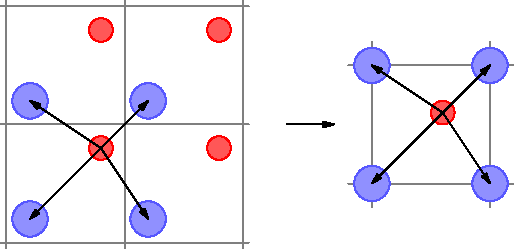
\includegraphics[width = 0.56\textwidth]{img/cryst-cvp}}%
	{\caption{键长计算和 CVP 的等价性}\label{fig:cryst-cvp}}
\end{figure}

CVP 在当代密码学研究中意义重大\footnote{%
	事实上,\emph{decryst} 这一名字除了“\textbf{de}crypt your \textbf{cryst}al
	structure”的表层含义之外,还暗示着晶体学(\textbf{cryst}allography)
	和密码学(\textbf{crypt}ography)两个领域之间因 CVP 而形成的联系。%
},在很大程度上是因为其计算复杂度随着所用向量空间的维数急剧增长,即使用量子
计算机求解也一样\parencite{micciancio2009};而如果对所用的向量空间能找到
一个尽量短且接近正交的基向量组,其计算会容易很多。晶体学中所用向量空间的
维数常常不超过 3,因此 CVP 的计算复杂度并不构成严重问题,但我们仍须进行%
\myterm{晶格归约},因为本文所用的细碰撞检测算法假定离位移向量最近的格点
一定不会在包围此向量的晶胞之外,而这意味着我们须要选取合适的晶胞
(其一反例见图 \ref{fig:bad-cell}\footnote{%
	有必要指出的是,其中按最近格点对平面进行划分得到的正是 Voronoi 图
	(参考第 \ref{ssec:narrow-discus} 小节)。%
})。

\begin{figure}[htbp!]\bfcmd
\setlength{\columnsep}{2.5em}
\begin{floatrow}
	\ffigbox[0.42\textwidth]{%
		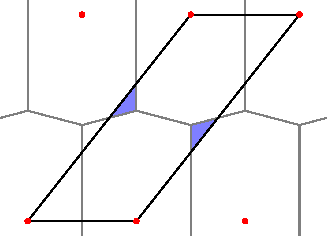
\includegraphics[width = 0.32\textwidth]{img/bad-cell}
	}{\caption[一种不好的晶胞选择]{%
		一种不好的晶胞选择,其使得离深色区域中任意点最近的格点在晶胞之外
		(浅色的分界线表示按离各个点最近的格点对平面进行的划分)%
	}\label{fig:bad-cell}}
	\ffigbox[\FBwidth]{%
		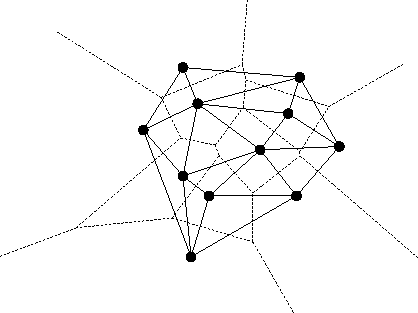
\includegraphics[width = 0.45\textwidth]{img/voro-delau}
	}{\caption[Voronoi 图和 Delaunay 三角化之间的对偶关系]{%
		Voronoi 图(虚线)和 Delaunay 三角化(实线)之间的对偶关系
		(图引自文献 (\cite[196]{berg2008}))%
	}\label{fig:voro-delau}}
\end{floatrow}
\end{figure}

在选取合适的晶胞之后便可以计算键长:首先计算两原子之间的位移向量,然后计算
包围位移向量的晶胞中所有格点和位移向量的距离里最短的一个。另一种常用算法%
\parencite{attfield1999, grudinin2010}是构造一个原子在原子对所属晶胞的所有
紧邻晶胞中的副本,然后计算这一原子以及上述所有副本到另一原子之间的距离中
最短的一个。显然,这里的算法明显快于后一种算法:对于三维晶格,
后一种算法须要计算距离 27 次,而这里的算法只需 8 次。

此外本人注意到对于分数坐标下 $l^1$ 范数
\begin{equation}
	|\upDelta x| + |\upDelta y| + |\upDelta z| < 1 / 2
\end{equation}
的位移向量,\textcite{kshirsagar2015}直接以位移向量的长度作为键长,
但本人未能找到其正确性的证明。\emph{SHELX}\parencite{sheldrick2010}%
中也采用了这一算法,但其说明中似乎未对位移向量的 $l^1$ 范数进行明确的限制。

\subsection{一种原子重叠评估函数}\label{ssec:eval-func}

如第 \ref{sec:atom-bump} 节所述,正空间法中出现原子重叠问题的原因在于 Bragg $R$
因子小的晶体模型仍可能发生原子重叠,而原始的全局最优化中也并未考虑原子重叠;
因此,如果以某种方式在最优化中考虑原子重叠,就可以自动地排除存在原子重叠的模型。
一种在全局最优化中考虑原子重叠问题的思路是修改最优化问题的约束条件,从而使得
生成的晶体模型总是那些不发生原子重叠的;然而这样会使最优化的操作变得十分繁琐,
其中最重要的原因是在上述约束条件下可行模型的集合将被分割为许多互相孤立的碎片,
这将和最优化算法中对自变量随机地进行连续微扰的做法发生冲突,
使得最优化的效率显著降低。

考虑到上述问题,本人采用了修改目标函数的做法:既然只用 $R$ 因子不能很好地排除
存在原子重叠的晶体模型,那就在目标函数中明确地加入一个对存在重叠的模型进行惩罚的
评估函数,从而使得最优化算法自动地倾向于生成无重叠的解模型。在最优化算法中,
目标函数往往被看成某种物理系统的势能函数,因此优化目标函数就是降低系统的势能;
仿照这一思路,这里的评估函数被设计为基于一个两体势
\vspace{\slop{0.3em}}
\begin{equation}
	C = \sum_{\{k_0, k_1\}} c(k_0, k_1)\mccomma\label{eq:two-body}
	\vspace{\slop{0.2em}}
\end{equation}
其中 $k$ 为晶胞中原子的编号;对势函数 $c$ 被定义为
\begin{equation}
	c(k_0, k_1) = f(d(k_0, k_1) \big/ d_0(k_0, k_1))\mccomma
\end{equation}
其中 $d$ 和 $d_0$ 分别为原子对的实际键长和正常键长。
$f$ 是一个分段线性函数,其控制节点为
\begin{equation}
	f(0) = f(0.75) = 1\mccomma f(0.875) = f(+\infty) = 0\mcscolon
\end{equation}
其形态被设计为和 Lennard-Jones 势的相似,但斜率更加平缓(图
\ref{fig:eq-eval-2})。注意到我们只在两原子间键长为正常键长的 0.875 倍时开始
考虑它们的相互作用,各原子的碰撞检测半径(参考第 \ref{ssec:cryst-sap} 小节)
可以按下式计算:
\begin{equation}
	r(k) = 0.875 q(k) r_0(k)\mcstop
\end{equation}

上述的两体势 $C$ 显然满足等效点系对称性(参考第 \ref{ssec:ep-sym} 小节),
因此可以利用 (\ref{eq:ep-sym}) 式加速计算。对于总原子数 $n$ 较大的晶胞,
因为可能有更多的原子对发生重叠,$C$ 的平均值也会比较大。为了处理这一问题,
实际算法中使用的评估函数被定义为
\begin{equation}
	B = \min(C/n, 1)\mccomma
\end{equation}
其取值上限被强行设定为 1 的原因是当 $C = n$ 时,平均每个原子会和两个原子
全面重叠,而此时可以认为相应的晶体模型是极不合理的。注意到 $B \in [0, 1]$,
如果能找到 Bragg $R$ 因子的一个上界 $\nu$,就可以将目标函数定义为
\begin{equation}
	E = \mu B + (1 - \mu) R/\nu\quad(\mu \in [0, 1])\mccomma
\end{equation}
这样对组合因子 $\mu$ 的任何值都有 $E \in [0, 1]$。事实上,
如果计算的衍射谱和实际谱都使用归一化的峰强\footnote{%
	许多从粉末衍射数据求解晶体结构的软件使用的正是归一化的峰强;本人开发的
	\emph{decryst} 也是如此,因此后者可以使用 (\ref{eq:obj-func}) 式。%
},那么可以得到
\begin{equation}
	R = \sum_i |I_{\text{obs}, i} - I_{\text{calc}, i}|
		\Big/ \sum_i I_{\text{obs}, i}
	= \sum_i |I_{\text{obs}, i} - I_{\text{calc}, i}| = 2D
	\mccomma\label{eq:total-var}
\end{equation}
其中 $D \in [0, 1]$ 为看作离散概率测度的两衍射谱之间的总变差距离%
\parencite{levin2008};于是可知 $\nu = 2$,并得到目标函数的实际公式
\begin{equation}
	E = \mu B + (1 - \mu) D = \mu B + (1 - \mu) R/2
	\mcstop\label{eq:obj-func}
\end{equation}

\subsection{原子重叠排除机制的测评}\label{ssec:cd-eval}

本小节涉及的测试代码可从 \emph{decryst} 的项目主页自由获取:%
\url{https://gitea.com/CasperVector/decryst};测试数据(含测试结构的晶胞参数、
等效点系组合和缩放因子)以及图 \ref{fig:pso-bump} 所对应的结构数据\footnote{%
	AMCSD 数据库结构代号:0005558。%
}可以从文献\parencite{liu2017}的补充材料中获取。因为 SAP 算法的常数因子较大
(从下文中可见),为了保证结果的一致性,这里只在具有最小 $R/ar$ 值(参考第
\ref{ssec:cryst-geom} 节)的单个坐标轴上使用了 SAP 算法。

为了测试第 \ref{ssec:cryst-sap}--\ref{ssec:ep-sym} 小节算法的有效性,本人从
美国矿物学家晶体结构数据库(American Mineralogist Crystal Structure Database,
简称 AMCSD;参考 \cite{downs2003})中获取了若干个不同复杂度的结构,并对每个
结构通过为独立原子赋予随机坐标的方式生成了 10000 个晶体模型。对于每个结构,
本人计算了在使用或不使用 (\ref{eq:ep-sym}) 式时(分别对应于 $N_\text{max}$
和 $N_\text{orig}$)每个模型所需细检测次数的上限,并统计了每个模型实际的细检测
次数($N_\text{real}$)和碰撞原子对数($N_\text{eff}$)的平均值和标准差,如表
\ref{tbl:cd-count} 所述。从表中可见,(\ref{eq:ep-sym}) 式和 SAP
都极大地减少了测试结构中需要细检测的原子对数。

\begin{table}[htbp!]\bfcmd
\ttabbox[0.75\textwidth]{\begin{tabular}{
	crrrrS@{\extracolsep{0.75em}}S
}\toprule
	ID &	$n$ &	$m$ &	$N_\text{orig}$ & $N_\text{max}$ &
	{$N_\text{real}$} &	{$N_\text{eff}$} \\\midrule
	0005558 &	24 &	5 &	276 &	105 &	50(3) &	8(3) \\
	0015840 &	64 &	8 &	2016 &	476 &	212(8) &	10(4) \\
	0009272 &	64 &	8 &	2016 &	476 &	218(24) &	43(22) \\
	0009563 &	90 &	10 &	4005 &	845 &	350(22) &	23(8) \\
	0002630 &	126 &	14 &	7875 &	1659 &	550(9) &	29(8) \\
	0000427 &	152 &	20 &	11476 &	2830 &	581(32) &	40(9) \\
	0000447 &	160 &	4 &	12720 &	630 &	227(11) &	8(3) \\\bottomrule
\end{tabular}}{\caption[碰撞检测算法的有效性测评]{%
	碰撞检测算法的有效性测评:ID 为测试结构在 AMCSD 中的代号;$n$ 和 $m$ 分别为
	晶胞中的总原子数和独立原子数;$N_\text{max}$ 和 $N_\text{orig}$ 分别为每个
	模型在用或不用 (\ref{eq:ep-sym}) 式时所需的细检测次数;$N_\text{real}$ 和
	$N_\text{eff}$ 分别为每个模型实际的细检测次数和碰撞原子对数。%
}\label{tbl:cd-count}}
\end{table}

为了测试上文中算法的性能,对于上述的每个测试结构,本人在不同条件下执行了一个测试
程序,每个条件下测试了 250 组晶体模型,每组由 250 个通过为独立原子赋予随机坐标
的方式生成的模型构成:
\begin{itemize}
	\item ($t_\text{void}$)不进行任何碰撞检测,只生成随机的晶体模型;
		该条件下度量的是测试程序本身的时间开销。
	\item ($t_\text{bn}$)无 SAP,只使用 (\ref{eq:ep-sym}) 式筛选原子对,
		细检测步骤被设为空指令;该条件下度量的是只使用 (\ref{eq:ep-sym})
		式进行粗检测的时间开销。
	\item ($t_\text{bN}$)无 SAP,只使用 (\ref{eq:ep-sym}) 式筛选原子对,
		但正常执行细检测步骤;该条件下度量的是只使用 (\ref{eq:ep-sym})
		式进行完整碰撞检测的时间开销。
	\item ($t_\text{Bn}$)使用 (\ref{eq:ep-sym}) 式和 SAP 筛选原子对,
		但细检测步骤被设为空指令;该条件下度量的是同时使用
		(\ref{eq:ep-sym}) 式和 SAP 进行粗检测的时间开销。
	\item ($t_\text{BN}$)完全的碰撞检测;该条件下度量的是使用
		(\ref{eq:ep-sym}) 式和 SAP 进行完整碰撞检测的时间开销。
	\item ($t_\text{orig}$)不使用 (\ref{eq:ep-sym}) 式或 SAP,
		但正常执行细检测步骤;该条件下度量的是逐对算法的时间开销。
\end{itemize}

对以上每种条件,本人在 Intel i7-3720QM CPU 上收集了测试程序在每组模型上所花费
时间的平均数和标准差,并将其除以每组的模型数,结果如表 \ref{tbl:cd-time} 所述。
从表中可见,对于各个复杂度的测试结构,第 \ref{ssec:cryst-sap}--\ref{ssec:ep-sym}
小节的算法都极大地降低了碰撞检测所花费的总时间;而且随着晶胞中原子数的增加,
这些算法和逐对算法相比的优势体现得更加显著。有必要强调的是,从表中也可以注意到,
虽然 SAP 是 $O(n\log n)$ 的算法,但是其常数因子较大(参考第 \ref{ssec:cryst-sap}
小节中归并排序和快速排序的比较),因此对于较小的晶胞而言只使用 (\ref{eq:ep-sym})
式进行粗检测可能在性能上会更有利。

\begin{table}[htbp!]\bfcmd
\sisetup{table-number-alignment = center}
\ttabbox{\begin{tabular}{
	cS[table-format = 1.5]@{\extracolsep{0.5em}}
	S[table-format = 2.5]@{\extracolsep{0.5em}}
	S[table-format = 3.4]@{\extracolsep{0.5em}}
	S[table-number-alignment = center-decimal-marker]@{\extracolsep{0.75em}}
	S[table-number-alignment = center-decimal-marker]@{\extracolsep{0.75em}}
	S[table-number-alignment = center-decimal-marker]
}\toprule
	ID &	{$t_\text{void}$} &	{$t_\text{bn}$} &	{$t_\text{bN}$} &
	{$t_\text{Bn}$} &	{$t_\text{BN}$} &	{$t_\text{orig}$} \\\midrule
	0005558 &	0.88(7) &	1.19(7) &	7.4(2) &
	8.0(2) &	10.9(3) &	17.6(5) \\
	0015840 &	1.8(1) &	3.2(1) &	31.8(8) &
	30.6(7) &	44(1) &	135(2) \\
	0009272 &	2.3(2) &	3.6(1) & 	31.4(4) &
	34.3(6) &	47(2) &	130(2) \\
	0009563 &	2.76(7) &	5.2(2) &	54.0(8) &
	57.3(6) &	78(1) &	257(3) \\
	0002630 &	3.6(1) &	8.0(2) &	105(1) &
	90(1) &	121(1) &	496(5) \\
	0000427 &	4.2(1) &	12(1) &	180(6) &
	91(2) &	124(3) &	727(7) \\
	0000447 &	3.8(1) &	5.6(2) &	46.2(6) &
	83(2) &	98(2) &	886(11) \\\bottomrule
\end{tabular}}{\caption[碰撞检测算法的性能测评]{%
	测试程序在每个模型上花费的时间(\si{\micro\second})。
	$t_\text{void}$:只生成模型;
	$t_\text{bn}$:使用 (\ref{eq:ep-sym}) 式;
	$t_\text{bN}$:(\ref{eq:ep-sym}) 式和细检测;
	$t_\text{Bn}$:(\ref{eq:ep-sym}) 式和 SAP;
	$t_\text{BN}$:(\ref{eq:ep-sym}) 式、SAP 和细检测;
	$t_\text{orig}$:使用逐对算法。%
}\label{tbl:cd-time}}
\end{table}

为了测试第 \ref{ssec:eval-func} 小节中原子重叠评估函数的有效性,本人利用
同一小节中的目标函数 $E$ 对 \ce{PbSO4} 结构进行了求解:对于组合因子
$\mu = 0, 0.01, 0.02, \cdots, 0.5$ 的每个值\footnote{%
	上限取 0.5 是考虑到我们的最终目标是结构测定。%
},本人利用全局最优化算法生成了 1000 个随机的解模型,
并统计了它们的 $(D, B)$ 分布,如图 \ref{fig:db-distrib-1} 所示。
由图可见正确解的 $D = R/2$ 值并不是最低的,而 $D$ 值最低的解中都有严重的
原子重叠问题,这正好解释了第 \ref{sec:atom-bump} 节提到的通过最小化
$R$ 因子求解 \ce{PbSO4} 结构得到的多数是错误解的现象。

\begin{figure}[htbp!]\bfcmd
\ffigbox{%
	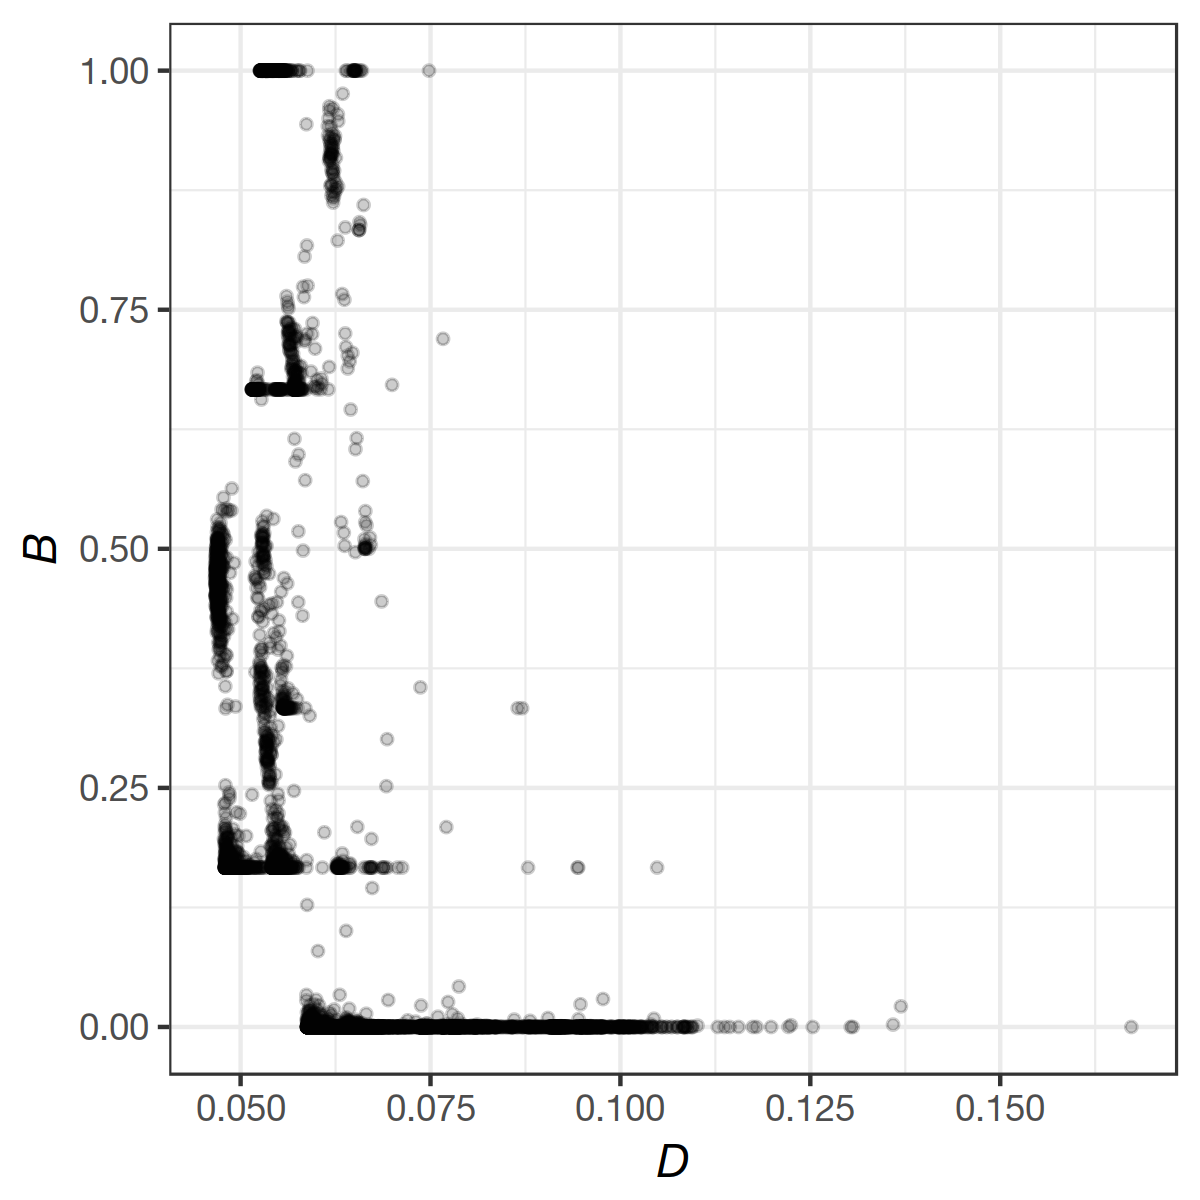
\includegraphics[width = 0.6\textwidth]{img/db-distrib-1}%
}{\caption[\ce{PbSO4} 随机解模型的 $(D, B)$ 分布]{%
	$\mu = 0, 0.01, 0.02, \cdots, 0.5$,每个 $\mu$
	值所对应 1000 个解模型的总体 $(D, B)$ 分布%
}\label{fig:db-distrib-1}}
\end{figure}

考虑到 $D$ 和 $B$ 都是原子坐标的连续函数,且两者都在和晶胞兼容的对称操作
之下保持不变,因为正确解的 $D = R/2 = 0.0642$、$B = 0$,
根据上图可以假定所有正确\footnote{%
	所有由对称操作所联系的模型都视为同一模型,
	而只在原子坐标上有细微差别的模型也视为等价。%
}的解模型都满足 $D < 0.12$、$B < 0.05$。为了
验证这一判据,本人生成了 100 个随机的满足判据的解模型,其中 $\mu \in [0, 0.5]$
为随机选取;在人工检查每个解之后,可以发现其中 99 个是正确的,而唯一错误解(图
\ref{fig:verify-fail})的 $D = 0.0814$(所有 100 个解中最大,次大值为 0.0705)。
本人由此假定一个解正确的充分必要条件为其 $D < 0.075$、$B < 0.05$,并统计了每个
$\mu$ 值所对应 1000 个解中正确解的比例,如图 \ref{fig:db-distrib-2} 所示。由图
可见,上述的评估函数在最优化的过程中有效地排除了 \ce{PbSO4} 的不合理晶体模型。

\begin{figure}[htbp!]\bfcmd
\vspace{\slop{0.3em}}
\setlength{\columnsep}{3em}
\begin{floatrow}
	\ffigbox[0.33\textwidth]{%
		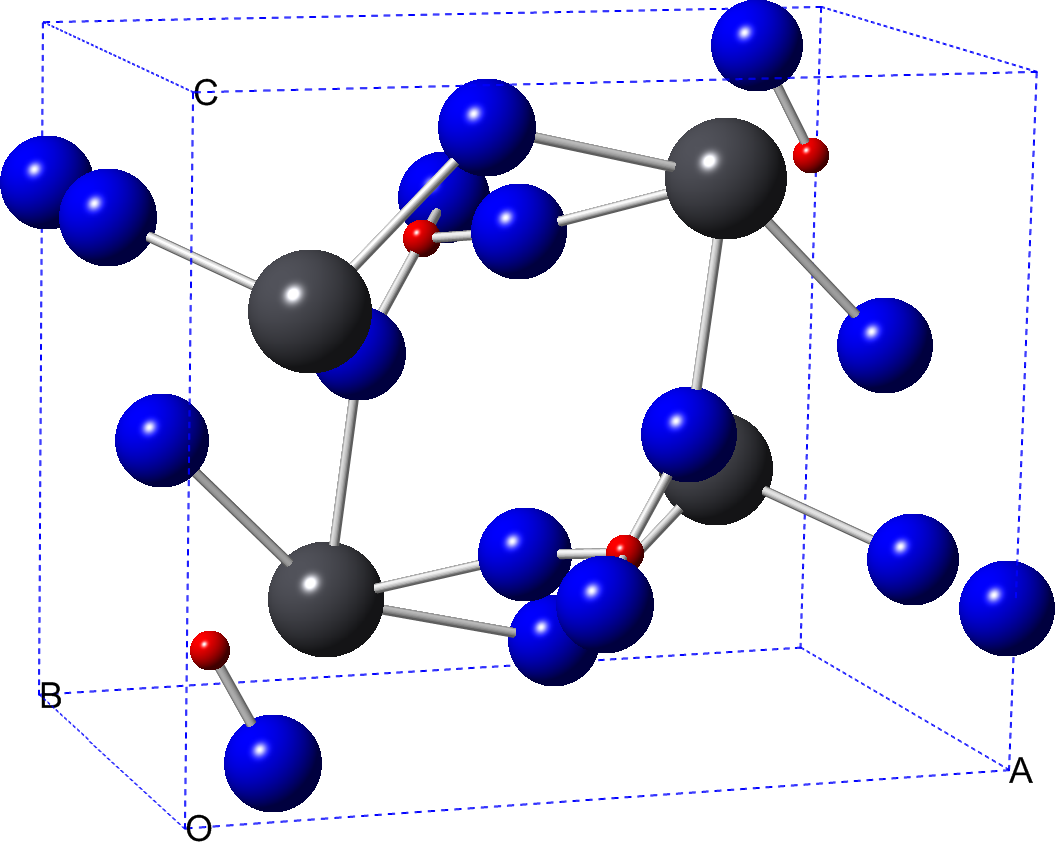
\includegraphics[width = 0.3\textwidth]{img/verify-fail-1}
	}{\caption[一个指标几乎合理的错误解]{%
		一个指标几乎合理的错误解($D = 0.0814$,$B = 0$)
	}\label{fig:verify-fail}}
	\ffigbox[\FBwidth]%
		{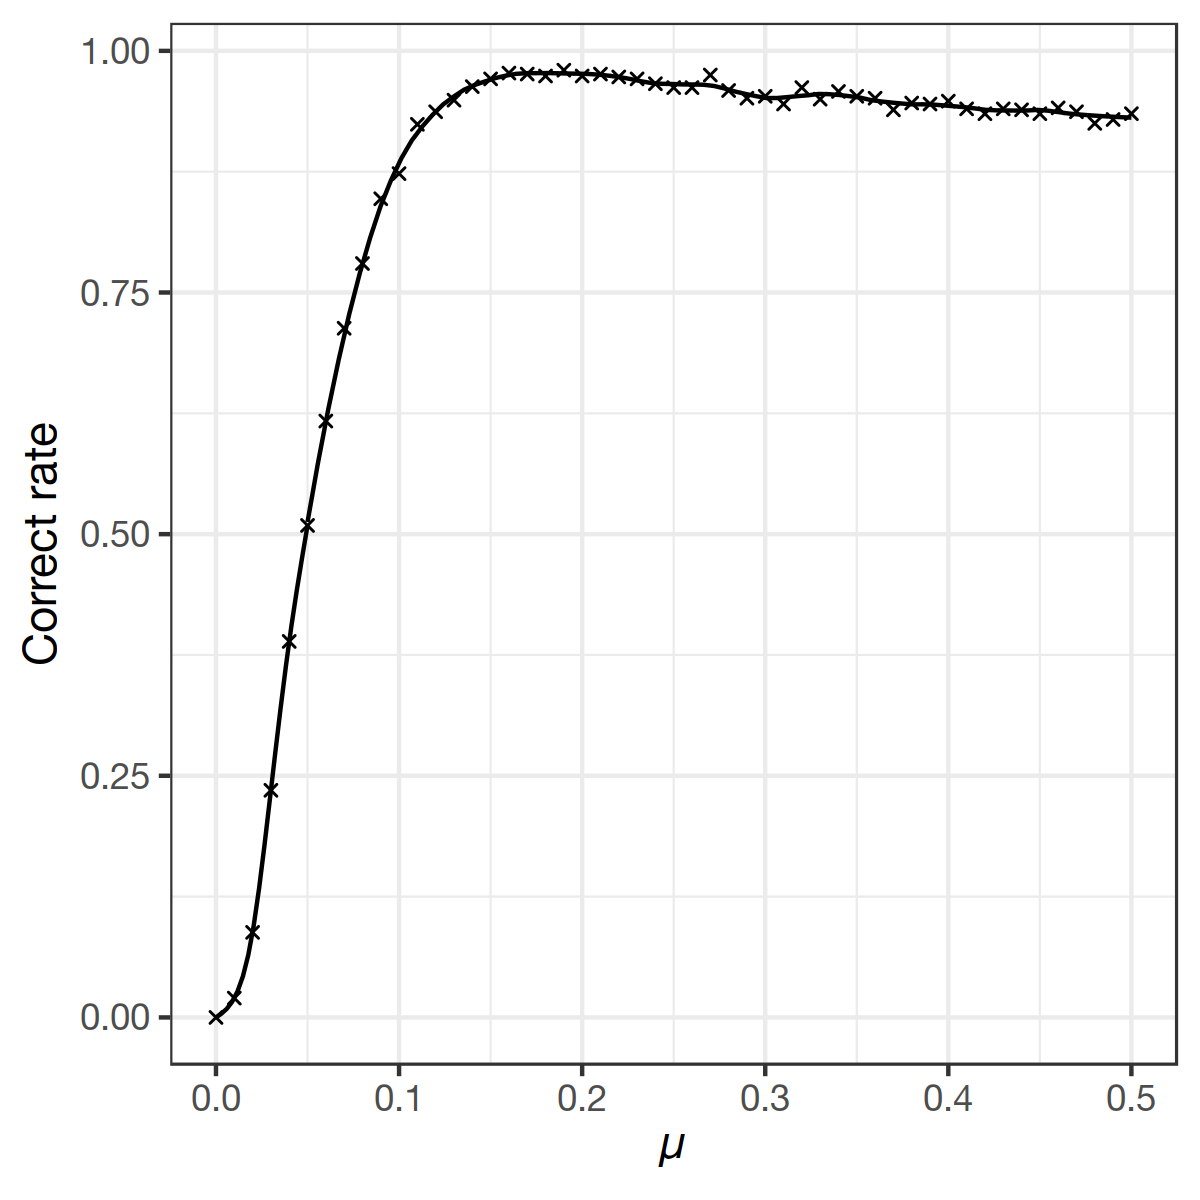
\includegraphics[width = 0.5\textwidth]{img/db-distrib-2}}%
		{\caption{不同 $\mu$ 值所对应解的实验正确率}\label{fig:db-distrib-2}}
\end{floatrow}
\vspace{\slop{-0.3em}}
\end{figure}

\section{讨论和小结}
\subsection{关于细碰撞检测正确性的讨论}\label{ssec:narrow-discus}

如第 \ref{ssec:cryst-cvp} 小节所述,本文中计算键长的算法假定已经选取合适的
晶胞,从而使得离位移向量最近的格点一定不会在包围此向量的晶胞之外。然而,能这样
做的条件是对每一个晶格都至少存在一个满足要求的晶胞,但本人未能找到这一条件的
严格证明。希望理论工作者能证明或证伪这一条件,并(如果条件是正确的)给出一种构造
合适晶胞的算法;另一方面,如果这一条件是错误的,本文中的细检测算法将不得不搜索
更多的近邻晶胞以寻找离位移向量最近的格点,但本文中的粗检测算法将不需改动。

考虑到在二维情形下,晶胞出现类似于图 \ref{fig:bad-cell} 中问题的前提是其一对对边
在正交投影下没有重叠(图 \ref{fig:voro-trans}),而晶格归约中的 Seeber 算法%
\parencite{engel1986}正好会排除这种情形,后者可能会在上述问题的研究中
有一定的启发意义。另一种或许具有可行性的研究思路是利用 Voronoi 图%
\parencite[147-171]{berg2008}和 Delaunay 三角化\parencite[191-218]{berg2008}%
之间的对偶关系(图 \ref{fig:voro-delau}):本人猜想,格点的 Delaunay 三角化%
\parencite{caroli2016}可能满足离任意点最近的格点是其一包围单纯形的顶点;
在此基础之上,通过适当拼接这些单纯形,或许就可以得到满足要求的晶胞。
此外在二维情形下,Delaunay 三角化会最小化所有三角形中的最大内角,
而这似乎也和晶格归约有一定的内在关联。

\begin{figure}[htbp!]\bfcmd
\ffigbox%
	{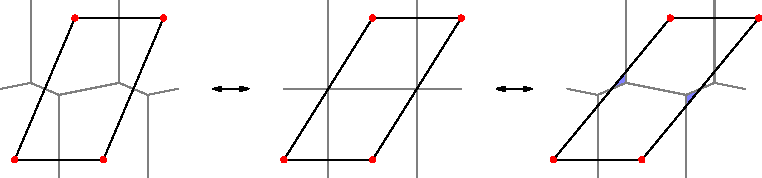
\includegraphics[width = 0.96\textwidth]{img/voro-trans}}%
	{\caption{格点的 Voronoi 图随晶胞参数的变化}\label{fig:voro-trans}}
\end{figure}

最后有必要指出,如果第 \ref{ssec:cryst-cvp} 小节中对 $l^1$ 范数小于 $1/2$
的位移向量计算键长的简便算法被证明是正确的,那么我们将能大幅度地进一步减少
计算短距离原子对键长所花费的时间。尽管上述简便算法尚无严格证明,但本人倾向于
认为其是正确的,只是需要一定的限制条件,包括合适的晶胞选择\footnote{%
	本人在某些限制条件下对随机产生的晶胞进行了测试(具体代码参考第
	\ref{ssec:decr-arch} 小节中的说明),未能找到这一简便算法的反例。
	随机测试显然不能取代严格证明,但本人基于此测试猜想这一算法应该正确。%
}(例如图 \ref{fig:bad-cell} 中的晶胞便会使上述简便算法出错)。另外,如果在某些
应用场景下,对于原子对没有进行除了 (\ref{eq:ep-sym}) 式之外的筛选,那么长距离原
子对将不能被充分筛除,因此在这些应用场景中上述算法带来的性能提升将较为有限。

\subsection{其它讨论}

(\ref{eq:ep-sym}) 式并未彻底利用特殊位置的对称性:例如在图 \ref{fig:eq-eval-1}
中因为 $c(00, 10) = c(00, 11)$、$c(00, 12) = c(00, 13)$,
总的两体势事实上可以被进一步归约为
\begin{equation}
	C = c(00, 01) + 4c(00, 10) + 2c(00, 12) + 2c(10, \{01, 11, 12, 13\})\mcstop
\end{equation}
如果这样的归约能自动进行,那么 $C$ 的计算将能进一步简化;然而这样很可能将需要一
个比 (\ref{eq:ep-sym}) 式中的 $(\delta_{j_0}n_{i_0} + \delta_{j_1}n_{i_1}) / 2$
复杂得多的原子对多重度计算公式,而后者本身的计算开销未必能被其对
$C$ 的简化所带来的性能提升所补偿。

在表 \ref{tbl:cd-time} 中,尽管“0000447”是总原子数 $n$ 最大的结构,
但其 $t_\text{bN}$ 却小于 $t_\text{BN}$,这是因为其独立原子数 $m$ 太小,
导致其晶体模型中绝大多数原子对被 (\ref{eq:ep-sym}) 式筛除。此外尽管如第
\ref{ssec:cryst-sap} 小节所述,SAP 算法并不特别适用于成键关系大部分已知的结构,
但如果这类结构中的成键信息因故不须在碰撞检测中考虑时,其也可以用 SAP 来处理:在
表 \ref{tbl:cd-time} 中,“0015840”(其中唯一的分子晶体)的测试结果和“0009272”
的结果相差并不大,这在两结构的 $n$、$m$ 值都完全相同的背景之下不难理解。

更加复杂的两体势,例如 \textcite{bushmarinov2012}所用的势或者甚至吸引势,原则上
也是可以在实际的评估函数中使用的。第 \ref{ssec:eval-func} 小节中的对势 $c$ 只
仿照了 Lennard-Jones 势中的排斥部分,因为本人认为我们的目标是排除原子重叠,而
不是对原子之间的相互作用进行精确的建模。虽然如此,从第 \ref{ssec:cd-eval} 小节
可见,目前使用的评估函数应该至少对包括 \ce{PbSO4} 在内的一些简单结构是有效的,
而其在求解更复杂结构时的应用将在第 \ref{chap:decr-usage} 章中展示。

对于很复杂的结构,特别是独立原子数很大的结构,期望只使用 Bragg $R$ 因子和原子
重叠评估函数就能成功求解是不太现实的:在这些结构的晶体模型中,完全有可能存在一些
$R$ 因子合理且无明显原子重叠,但在成键类型、配位数、配位多面体形态、键价等等
方面有问题的模型。相应地,我们须要在结构测定中应用更多的\myterm{结构验证}%
(structure validation;参考 \cite{spek2003})手段,而第 \ref{chap:decr-usage}
章将给出一些通过人工方式进行结构验证的例子;但为了实现使结构测定更加自动化的
目标,我们最终须要做的显然是将更多的结构验证技术自动化地引入结构测定中。考虑到在
结构验证中很多测试都以结构中的成键关系为基础,可以认为第 \ref{ssec:cryst-sap}--%
\ref{ssec:ep-sym} 小节的算法应该会在这些方面的研究中发挥基础性的作用。

\subsection{本章小结}

针对晶体结构测定中的原子重叠问题,本人基于轴对齐包围盒(AABB)模型提出了
一种具有通用性的晶体学碰撞检测算法框架。为了处理成键关系总体未知的结构,
本人基于上述框架修改了 sweep and prune(SAP)算法,使之能以 $O(n\log n)$
的时间复杂度检测晶胞中的成键关系。考虑到在求解成键关系总体未知的结构时常常
使用等效点系组合(EPC)法,本人也提出了一种利用等效点系对称性极大降低碰撞
检测复杂度的算法,这一算法即使对于小晶胞也可以显著降低碰撞检测的时间开销。
基于以上算法,本人提出了一种针对晶胞中原子重叠状况的评估函数,其可以用于
在正空间法的全局最优化步骤中实时地排除存在原子重叠的晶体模型;此外,
上述算法对于晶胞中配位多面体、原子键价等等的计算也具有重要的意义。

\begin{rquote}{}
	即得易见平凡,仿照上例显然;留作习题答案略,读者自证不难。\\
	反之亦然同理,推论自然成立;略去过程 Q.E.D.,由上可知证毕。
\end{rquote}
\rightline{——《\emph{西江月·证明}》(摘自互联网)}

% vim:ts=4:sw=4
